\section{DRX}
Métodos de difração de raios-X (DRX) são métodos para determinação da
estrutura cristalina \cite{bookMaterialsCharacterizationYang}. O método 
baseia-se na identificação dos compostos através de sua estrutura 
cristalina e não por sua composição. Ou seja, diferentes compostos 
(ou fases), com a mesma composição podem ser identificados.

\subsection{Príncípio da Técnica}
O princípio baseia-se na geração de raios-X, atráves de eletrons de
alta velocidade acelerados por um campo de alta voltagem, que se colidem,
com um metal \cite{bookMaterialsCharacterizationYang}. A rápida desaceleração ocasionada pela colisão, permitem a
conversão da energia cinética em energia de radiação de raio-X. Desta forma
o compimento de onda $\lambda$ da radiação raio-X é relacionada com a tensão
dos eletrons (V), conforme descrito na equação \ref{eq:waveLenghtXRay}.

\begin{equation}\label{eq:waveLenghtXRay}
    \lambda = \frac{1.2398 * 10^{3}}{V} (nm)
\end{equation}

Uma vez que as ondas de raio X possuem energia elevada e curtos
comprimentos de onda, da ordem de magnitude dos espaçamentos atômicos, uma fração do feixe
de raios X se dispersa quando atinge uma amostra \cite{bookMaterialsScienceEngineeringCallister}.

Duas ondas de raio X com o mesmo comprimento de onda viajando na mesma direção
pode intereferir uma na outra dependendo da diferença de fase. Quando a diferença
de fase é de números inteiros de $\lambda$, ocorre uma intereferencia construtiva,
contudo, quando a intereferência é de $n \lambda/2$, ocorre a intereferência destrutiva
\cite{bookMaterialsCharacterizationYang}. Desta forma, feixes que incidem sobre sólidos
cristalinos serão difratados pelos planos cristalográficos, conforme indicado na figure
\ref{figureCristallographicPlanes}. As ondas desviadas não estarão em fase, a não ser que
atendam a equação \ref{eq:braggEquation}, sendo esta a equação de Bragg.

\begin{equation}\label{eq:braggEquation}
    n\lambda = 2d\sin\theta
\end{equation}

\begin{figure}[ht]
    \center
    \begin{minipage}{13cm}
     \caption{Difração de Bragg por planos cristalográficos.}\label{figureCristallographicPlanes} 
     \frame{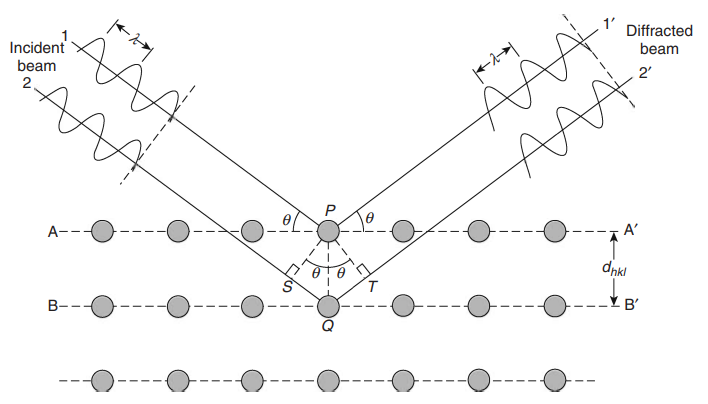
\includegraphics[scale=0.7]{figures/drx/bragDiffractions.png}}
     \legend{\citefonte{bookMaterialsCharacterizationYang}.}
     \end{minipage}
\end{figure}

Sete diferentes combinações dos parâmetros de rede. Cada uma dessas combinações
constituem um \textbf{sistema cristalino} \cite{pptDifracaoRaioXAntonioCarlos},
sendo estes apresentados na figure \ref{figureCrystalSystems}.

\begin{figure}[ht]
    \center
    \begin{minipage}{15cm}
     \caption{Sistemas Cristalinos.}\label{figureCrystalSystems} 
     \frame{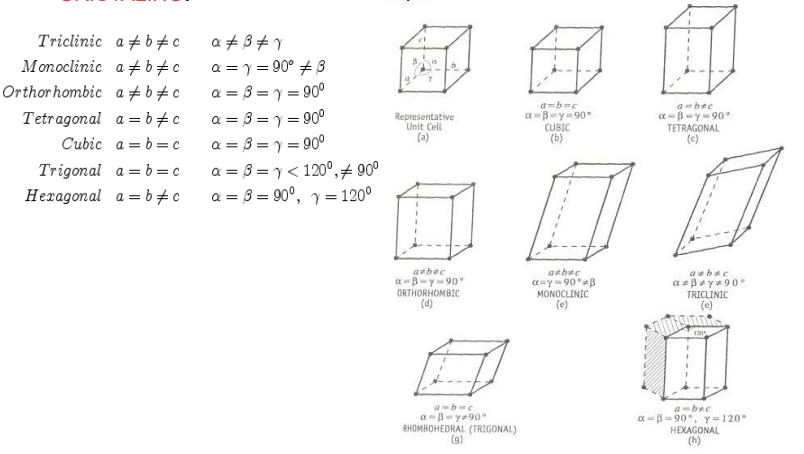
\includegraphics[scale=0.7]{figures/drx/cristallynesSystens.png}}
     \legend{\citefonte{bookMaterialsCharacterizationYang}.}
     \end{minipage}
\end{figure}

Portanto, podemos obter o espaço entre planos atômicos de um cristal quando
inferência construtiva é detectada em um anglo incidente e um comprimento de onda
baseado na lei de Bragg. Utilizando a equação \ref{eq:cristalographicDistance} por exemplo,
podemos determinar a distância interplanar para um cristal cúbico, sendo
a o tamanho da aresta.

\begin{equation}\label{eq:cristalographicDistance}
        d_{hkl} = \frac{a}{\sqrt[]{h^2+k^2+l^2}}        
\end{equation}

Os índices de Miller ($h, k, l$) são vetores que unem dois pontos da rede cristalina,
portanto são a direção cristalográfica \cite{pptDifracaoRaioXAntonioCarlos}. Através
de operações matemáticas faz-se com que o vetor passe pela origem do sistema de coordenadas,
com posterior projeção do vetor em cada um dos três eixos, para que esta projeção seja
medida em termo de dos parâmetros da rede (a,b, c). Uma exemplo de um plano cristalográficos
é aprensetado na figura \ref{figure:cristalographicPlane}.

\begin{figure}[ht]
    \center
    \begin{minipage}{8cm}
     \caption{Exemplo de plnao cristalografico.}\label{figure:cristalographicPlane} 
     \frame{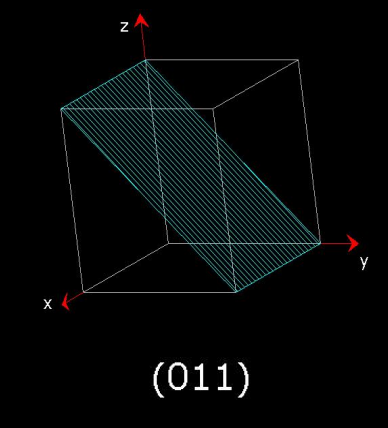
\includegraphics[scale=0.7]{figures/drx/crystalographicPlane.png}}
     \legend{\citefonte{pptDifracaoRaioXAntonioCarlos}.}
     \end{minipage}
\end{figure}

\subsection{Equipamento}

O difratômetro de raio X é o equipamento utilizado neste tipo de análise.
Inicialmente os raios X são produzidos um tubo de raio X,
conforme Figura \ref{figureXRayTube} geralmente em molibidênio ou cobre, 
em que é controlado o comprimento de onda pela diferênça de potencial no
tubo. 

\begin{figure}[ht]
    \center
    \begin{minipage}{12cm}
     \caption{Estrutura do tubo de raio X.}\label{figureXRayTube} 
     \frame{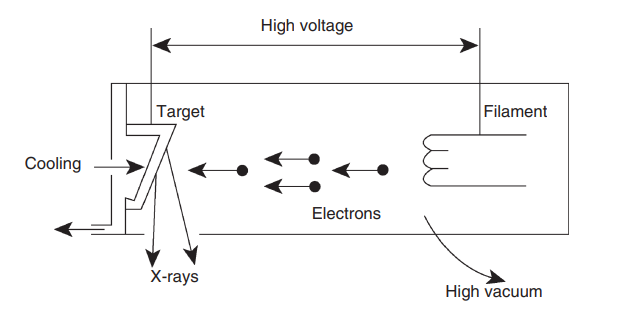
\includegraphics[scale=0.7]{figures/drx/xraytube.png}}
     \legend{\citefonte{bookMaterialsCharacterizationYang}.}
     \end{minipage}
\end{figure}

Os raiox X passam pelo colimador, que funciona para estreitar os feixe dos raios,
que então são incididos sobra a amostra que tem o ângulo de incidência
modificado a uma taxa determinada \cite{bookMaterialsCharacterizationYang}.
Os raios difratados detectados por um contador Geiger, sendo posteriormente gravados,
juntamente como o ângulo de incidência, formam um espectro da intensidade da difração
pelo ângulo incidente.

O esquema completo do sistema de difatrômetro de pó clássico é apresentado
na figura \ref{figurePptDifratometroPo}.

\begin{figure}[ht]
    \center
    \begin{minipage}{16cm}
     \caption{Difratômetro de pó clássico}\label{figurePptDifratometroPo} 
     \frame{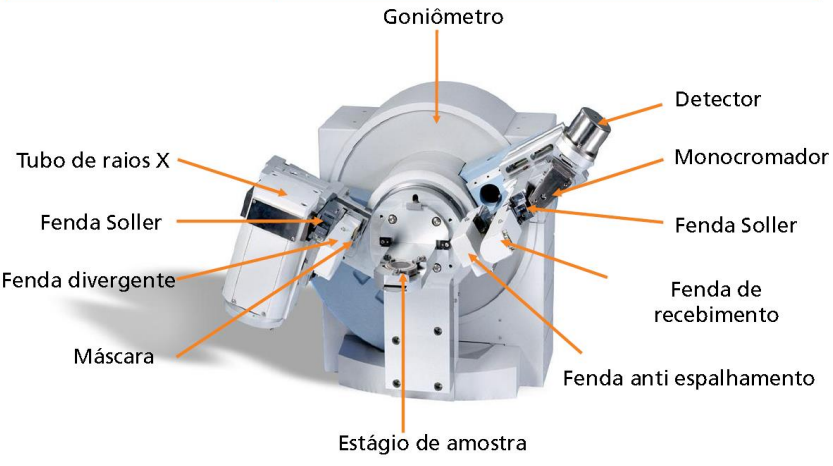
\includegraphics[scale=0.7]{figures/drx/DifratometroPoClassico.png}}
     \legend{\citefonte{pptDifracaoRaioXAntonioCarlos}.}
     \end{minipage}
\end{figure}

\subsection{Preparação da Amostra}
Quanto a preparação da amostra no método do pó, a amostra deve ser
homogeneizada e estar na forma de pó finamente disperso, com o objetivo
de preencher o porta-amostra, ficando a amostra rente ao plano superior
do porta-amostra. Exemplos de empacotamento da amostra no porta-amostra,
são apresentados na figura \ref{figureEmpacotamentoPortaAmostra}.

\begin{figure}[ht]
    \center
    \begin{minipage}{10cm}
     \caption{Tipos de empacotamento.}\label{figureEmpacotamentoPortaAmostra} 
     \frame{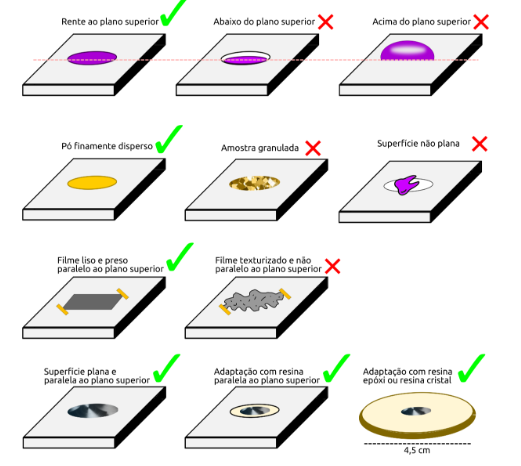
\includegraphics[scale=0.7]{figures/drx/TiposDeEmpacotamentoPortaAmostra.png}}
     \legend{\citefonte{webSiteCAIQUNB}.}
     \end{minipage}
\end{figure}

\subsection{Condições de Análise}
Para a realização da análise, as condições devem ser definidas, sendo elas:
\begin{itemize}
    \item Faixa de Ângulo 2$\theta$.
    \item Incremento (\textit{step})
    \item Velocidade de rotação (graus/min)
\end{itemize}

Ainda, deve ser observado as capacidades do equipamento como a tensão máxima
de operação, a correnta máxima e qual o material fonte de irradiação. Estes
parâmetros definem qual o comprimento de onda, que influi diretamente na intensidade
observada no difratograma.

\subsection{Tratamento dos Dados}

É comum que os dados resultantes da análise necessitem de tratamento. O objetivo
dos tratamentos podem ser para correção da linha de base, remoção de ruídos e
desconvolução (método de separação de picos sobrepostos).

\subsection{Avaliação dos Dados}

Uma vez que obtido o difratograma, as fases são identificadas por comparação
com o banco de dados obtidos no ICDD (\textit{International Center Diffraction
Data}) \cite{bookMaterialsCharacterizationYang}. O mesmo é valido para misturas,
onde as comparações são realizadas pelos padrões de cada componente. A avaliação
dos resultados podem ser realizadas por softwares,
sendo alguns destes:

\begin{itemize}
    \item Dffrac.EVA \cite{webSiteDiffracEva}.
    \item DAJUST \cite{articleDajust}.
    \item HighScore Plus \cite{webHighScorePlus}.
\end{itemize}

A análise do difratograma tem como objetivo obter informações
de intensidade, posição angular (2$\theta$), distância interplanar (d)
e o perfil no pico. Com estas informações, é possível determinar
o grau de cristalinidade com base em um padrão. Parâmetros de Rede e sistema
Cristalino também podem ser determinados, de acordo com a figura \ref{figureCristalineSistem}, 
onde encontram-se as equações necessárias para identificar
o sistema cristalino presente na amostra. Além destes, o tamanho de cristal também
pode ser determinado.

\begin{figure}[ht]
    \center
    \begin{minipage}{14cm}
     \caption{Distância interplanar para sistemas cristalinos.}\label{figureCristalineSistem} 
     \frame{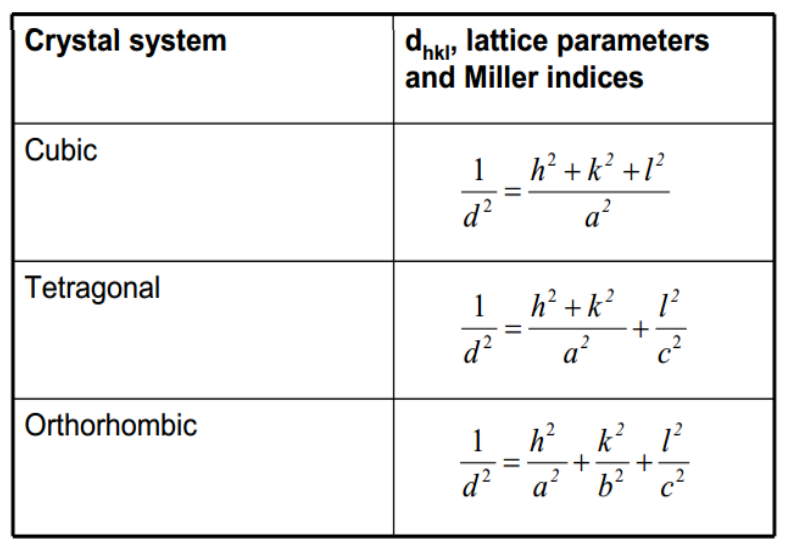
\includegraphics[scale=0.51]{figures/drx/distanciaInterplanar.png}}
     \legend{\citefonte{pptDifracaoRaioXAntonioCarlos}.}
     \end{minipage}
\end{figure}

\subsection{Comparação a literatura}

\subsubsection*{\textbf{Artigo I} - MCM-41 Ordered Mesoporous Molecular Sieves Synthesis
and Characterization.}

Para \citefonte{articleMelo1999} a difração de raio X foi realizada em
um difratômetro Siemens D500, usando radiação monocromática de CuK$\alpha$,
tendo como alcance angular de 1 até 10°, sendo a velocidade de rotação de
0.6°/min. 

O resultado da análise indica que os mesoporos da peneira moleuclar MCM-41,
pude, ram ser obtidos e permitiram a identificação dos picos relativos aos planos
(100), (110), (200) e (210), que são correspondentes a estrutura hexagonal. O
difratograma apresentado pelos autores pode ser observado na figura \ref{figure:difratogramArticleAguiar}.
Observou-se que há um maior pico relacionado ao plano (100) para síntese
em pressão autogênica comparada com síntese em refluxo, o que indica uma maior
organização dos canais dos mesoporos.

\begin{figure}[ht]
    \center
    \begin{minipage}{14cm}
     \caption{DRX para o MCM sintetizado em 48h.}\label{figure:difratogramArticleAguiar} 
     \frame{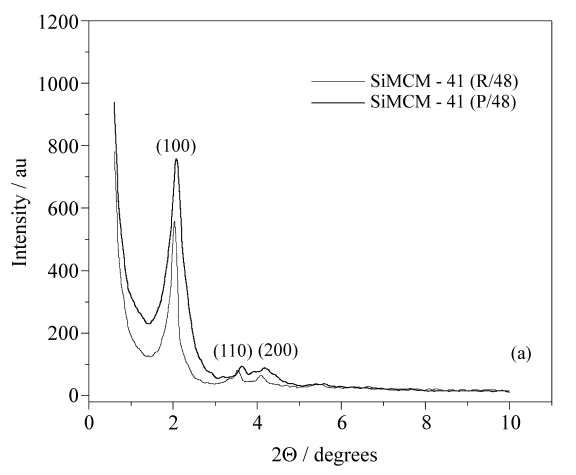
\includegraphics[scale=0.7]{figures/drx/difratogramaArtigoAguiar.png}}
     \legend{Fonte: \citefonte{articleMelo1999}.}
     \end{minipage}
\end{figure}

Além disso, o autor também realizou síntese do AlSiMCM-41, o difratograma obtido
para este material é apresentado na figura \ref{figure:AlSiMCM-41Aguiar2019}.
Em comparação do difratograma apresentado na figura \ref{figure:difratogramArticleAguiar}
com a figura \ref{figure:AlSiMCM-41Aguiar2019}, é que os picos para o material
que contém alumínio esta mais amplo e menos intenso, significando que o arranjo
hexagonal dos mesoporos estão menos organizados.

\begin{figure}[ht]
    \center
    \begin{minipage}{14cm}
     \caption{DRX para o MCM sintetizado em 48h.}\label{figure:AlSiMCM-41Aguiar2019} 
     \frame{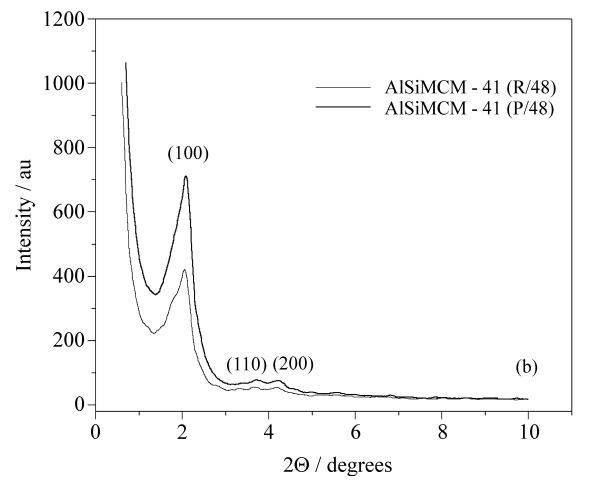
\includegraphics[scale=0.7]{figures/drx/AlSiMCM41_difratograma.png}}
     \legend{Fonte: \citefonte{articleMelo1999}.}
     \end{minipage}
\end{figure}

\subsubsection*{\textbf{Artigo II} - Performance of Al-MCM-41 nanospheres as catalysts for dimethyl
ether production.}

Os resultados de DRX obtidos por \citefonte{articleXRDBedoya2021} tiveram como condições de análise,
patrões de difração de raio X de baixo ângulo. Sendo os padrões gravados em um difratômetro Philips
X'Pert, como alcance de 2$\theta$ de 1.5° até 8°, usando \textit{Cu}K{$\alpha$} como fonte de 
radiação ($\lambda$ = 1.5406 \AA) em 45 kV e 30 mA. A descrição da nomenclatura das amostras
em função da concentração de Al é descrita na tabela \ref{tableBedoyaAlConcentration}.

\begin{table}[]
    \centering
    \begin{threeparttable}
    \caption{Concentração de alumínio por material.}
    \label{tableBedoyaAlConcentration}
    \begin{tabular}{cclll}
    \cline{1-2}
    Material      & Al (\% atômico) &  &  &  \\ \cline{1-2}
    Al-MCM41\_0.2 & 2,8             &  &  &  \\
    Al-MCM41\_0.3 & 3,2             &  &  &  \\
    Al-MCM41\_0.4 & 4,6             &  &  &  \\
    Al-MCM41\_0.5 & 3,7             &  &  &  \\ \cline{1-2}
    \end{tabular}
    \legend{Fonte: Autor.}
    \end{threeparttable}
    \end{table}

O difratograma obtido é apresentado na figura \ref{figureDifratogramBedoya2021}. O pico
em 2.3° é atribuido a difração do plano (100) de uma estrutura 2d-hexagonal organizada
associada a estrutura mesoporosa do MCM-41 (ICDD $\#$49-1712) \cite{articleXRDBedoya2021}. Os
picos de difração amplos e de baixa itensidade são atribuidos a estrutura bem definida
de baixas dimensões. Deste modo, o encolhimento da matriz hexagonal se deve a incorporação
do alumínio. O alargamento da difração do plano (100) é atribuido a mudança do ânglo da
Al-O-Si devido a incorporação do Alumínio, comparado com o ângulo da matriz Si-O-Si. A
ausência dos picos referentes ao planos (110) e (200) pode sugerir a mudança nos ângulos
de ligação do Al-O-Si. Também, é interessante notar que não houve modificação na estrutura
de acordo com a concentração do tetraetiloxissilano.

\begin{figure}[ht]
    \center
    \begin{minipage}{10cm}
     \caption{Padrões das difrações de raio X de baixo ângulo para as amostras de Al-MCM-41.}\label{figureDifratogramBedoya2021} 
     \frame{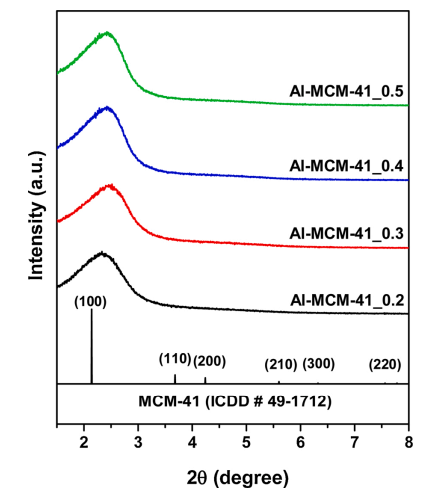
\includegraphics[scale=0.85]{figures/drx/difratogramBedoya2019.png}}
     \legend{\citefonte{articleXRDBedoya2021}.}
     \end{minipage}
\end{figure}

\subsubsection*{\textbf{Artigo III} - Ordered mesoporous molecular sieves synthesized
by a liquid crystal template mechanism.}

Segundo \citefonte{articleXRDKresge1992} o padrão de difração de raio X apresentado na figura \ref{figureXRDkresge1992},
é obtido atráves de sistema de difração automatizado Scintag PAD usando geometria 2$\theta$, com
radiação de CuK$\alpha$ ($\lambda$ = 1.5418 \AA) e um detector de energia dispersiva.

\begin{figure}[ht]
    \center
    \begin{minipage}{10cm}
     \caption{Padrão de difração para o MCM-41.}\label{figureXRDkresge1992} 
     \frame{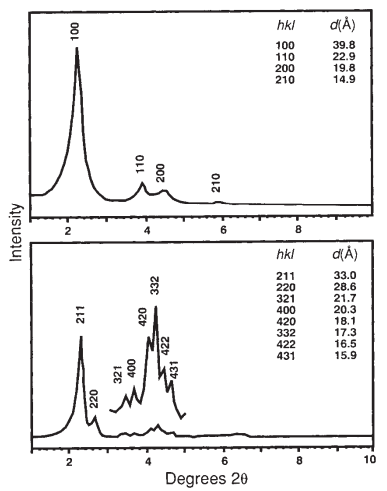
\includegraphics[scale=0.85]{figures/drx/kresge1992.png}}
     \legend{\citefonte{articleXRDKresge1992}.}
     \end{minipage}
\end{figure}

Os quatro picos observados no baixo ângulo 2$\theta$ pode ser indexado a estrutura
hexagonal da célula unitária com a $\approx$ 45 \AA (2$d_{100}/\sqrt[]{3}$).

\subsubsection*{\textbf{Artigo IV} - Síntese e apliacação dos materiais mesoporosos do tipo MCM-41 e
MCM-48 contendo metais (Ti ou Zn) em adsorção/fotocatálise do
corante azul de metileno.}

Para a obtenção do difratograma \citefonte{articledrxDaronch2019} utilizaram difratômetro
MiniFlex II Desktop X-ray \textit{Diffractometer} Rigaku. Obtendo como resultado o difratograma
apresentado na figura \ref{figureDRXDaronch2019}, em que os picos em 2 e 3° são devido
a uma estrutura cristalina. A presença de titânio no material Ti-MCM-41 é confirmada
devido ao pico 25 e 26°. Quanto ao sólidos obtidos no processo de preparação de materiais
Zn-MCM-41, também apresentaram cristalinidade em sua forma uma vez que possuem pico em 2° e 3°.
A presença de zinco nesta estrutura é confirmada pela com o pico em 32, 34 e 36°.

\begin{figure}[ht]
    \center
    \begin{minipage}{12cm}
     \caption{Difratogramas de raios X das amostras, onde (a) MCM-41, (b) Ti-MCM-41, (c) TiO2, (d) ZnMCM-41 e (e) ZnO.
     }\label{figureDRXDaronch2019} 
     \frame{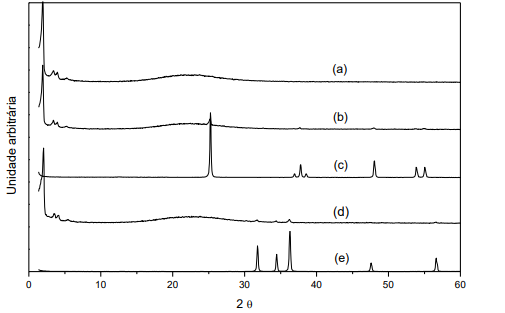
\includegraphics[scale=0.9]{figures/drx/daroschDifratograma2021.png}}
     \legend{\citefonte{articleXRDKresge1992}.}
     \end{minipage}
\end{figure}

\subsubsection*{\textbf{Artigo V} - Mesopore Molecular Sieve MCM-41 Containing Framework Aluminum.}

Na caracterização do MCM-41 contendo uma rede de alumínio por difração de raio X, \citefonte{articledrxLuan1995}
utlizando difratômetro Philips 1710 com radiação Cu K$\alpha$ (40 kV, 40 mA), com passo de
0.025° e 1 s por passo. 

\begin{figure}[ht]
    \center
    \begin{minipage}{9cm}
     \caption{Padrões de DRX do aluminosilicato calcinado MCM-41 com massa de Si/Al nas
     proporções de (a) 2.5, (b) 5, (c) 15, (d) 25, (e) 40 e (f) 60. (g) padrão DRX de MCM-41 puro.
     }\label{figureDRXLuan95} 
     \frame{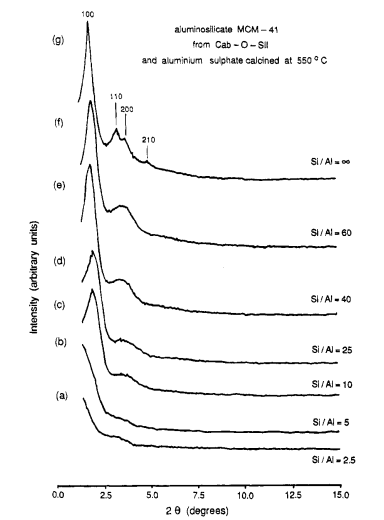
\includegraphics[scale=0.9]{figures/drx/xrddifratogramaLuan1995.png}}
     \legend{\citefonte{articledrxLuan1995}.}
     \end{minipage}
\end{figure}

Na figure \ref{figureDRXLuan95} os padrões de DRX das amostras com Si/Al > 10 calcinados a 550 °C (com
o objetivo de remoção das moléculas modelo), tem resolução melhores do que as amostras preparadas. o
pico (100) torna-se mais pontudo e mais intenso no caso de calcinação, embora os picos (110) e (200)
estão ainda mal definidos e sobrepostos para dar uma linha ampla singular.

\cite{articleDahl2019}.

